% ============================================================================
% Relatório do Trabalho Prático 2 - SCC0282 Recuperação de Informação
%
% Como compilar no Overleaf:
%   1. Envie este arquivo e a pasta "resultados/" com as duas figuras:
%        resultados/grafico_delta_lexical_semantico.png
%        resultados/grafico_comparacao_sistemas.png
%   2. Compilador: pdfLaTeX.
%   3. Procure por \completar no texto: são os pontos que dependem do grupo
%      (e-mails, revisão das notas da avaliação humana do RAG, uso de IA).
%
% Limite do enunciado: 20 páginas, sem contar as referências. Se o PDF passar
% do limite, troque "11pt" por "10pt" na linha do \documentclass.
% ============================================================================
\documentclass[11pt,a4paper]{article}

\usepackage[utf8]{inputenc}
\usepackage[T1]{fontenc}
\usepackage[brazil]{babel}
\usepackage{lmodern}
\usepackage[a4paper,margin=2.2cm]{geometry}
\usepackage{microtype}
\usepackage{amsmath}
\usepackage{booktabs}
\usepackage{graphicx}
\usepackage{enumitem}
\usepackage{xcolor}
\usepackage[font=small,labelfont=bf]{caption}
\usepackage{placeins}
\usepackage[hidelinks]{hyperref}

\graphicspath{{resultados/}{./}}
\setlist{nosep,leftmargin=1.4em}
\setlength{\emergencystretch}{2em}
\setlength{\parskip}{0.35em}
\setlength{\parindent}{0pt}
% Mantém tabelas e figuras perto do texto que as cita
\renewcommand{\topfraction}{0.9}
\renewcommand{\bottomfraction}{0.8}
\renewcommand{\textfraction}{0.08}
\renewcommand{\floatpagefraction}{0.85}
\setcounter{topnumber}{3}
\setcounter{bottomnumber}{2}
\setcounter{totalnumber}{5}

% Código, nomes de arquivos e de modelos
\newcommand{\cod}[1]{\texttt{#1}}
% Pontos que o grupo precisa completar antes da entrega (aparecem em vermelho no PDF)
\newcommand{\completar}[1]{\textcolor{red}{\textbf{[COMPLETAR: #1]}}}

\begin{document}

% ------------------------------- Cabeçalho ---------------------------------
\begin{center}
{\Large\bfseries Trabalho Prático 2: busca lexical, semântica e híbrida,\\[0.15em] reranking e RAG sobre o NFCorpus\par}
\vspace{0.7em}
{\normalsize Ana Paula de Abreu Batista (N\textsuperscript{o} USP 12688424) \quad
Italo Carlos Martins Bresciani (N\textsuperscript{o} USP 15461782)\par}
\vspace{0.3em}
{\small Bacharelado em Sistemas de Informação, ICMC, Universidade de São Paulo\\
SCC0282 Recuperação de Informação, 2\textsuperscript{o} semestre de 2026, Prof. Marcelo Manzato\\
\completar{e-mail da Ana Paula} \quad \completar{e-mail do Italo}\par}
\end{center}
\vspace{0.3em}

% ------------------------------- Introdução --------------------------------
\section{Introdução}

Sistemas modernos de Recuperação de Informação raramente dependem de uma única técnica. A busca lexical, baseada na correspondência exata de termos, é rápida e precisa quando a consulta usa as mesmas palavras dos documentos. A busca semântica, baseada em vetores densos, alcança documentos que tratam do mesmo assunto com outro vocabulário. Sobre os resultados dessas duas buscas costumam ser aplicados um modelo de reranking, mais preciso e mais caro, e um modelo de linguagem (LLM), que gera uma resposta a partir dos documentos recuperados (\emph{Retrieval-Augmented Generation}, RAG)~\cite{lewis2020}.

A motivação deste trabalho é entender, com evidências, o que cada um desses componentes acrescenta e onde cada um falha. O objetivo é desenvolver e avaliar, sobre a coleção NFCorpus, o pipeline completo
\begin{center}
\small documentos $\rightarrow$ pré-processamento e indexação $\rightarrow$ recuperação lexical + semântica $\rightarrow$ busca híbrida $\rightarrow$ reranking $\rightarrow$ seleção de contexto $\rightarrow$ LLM $\rightarrow$ resposta,
\end{center}
com avaliação quantitativa, análise por consulta e investigação de casos de sucesso e de falha.

Em resumo, os resultados no conjunto de teste são os seguintes. O BM25 sobre um índice invertido implementado do zero e a busca semântica têm desempenho global parecido (NDCG@10 de 0,3280 e 0,3167), mas acertam consultas diferentes. A fusão por RRF eleva o NDCG@10 para 0,3549. O reranking com cross-encoder acrescenta apenas 0,0015 e consome cerca de 97\% do tempo do pipeline. No experimento de RAG, o contexto recuperado eleva a fidelidade média das respostas de 0,7 para 1,9 (escala de 0 a 2), e a análise ponta a ponta mostra que a falha mais grave nasce na recuperação, e não na geração.

A Seção~\ref{sec:metodologia} descreve os componentes, a Seção~\ref{sec:avaliacao} o protocolo de avaliação, a Seção~\ref{sec:resultados} os resultados e as análises, e a Seção~\ref{sec:conclusao} as conclusões.

% ------------------------------- Metodologia -------------------------------
\section{Metodologia}
\label{sec:metodologia}

Cada documento é representado pela concatenação do título com o texto (\cod{title} + espaço + \cod{text}). Essa representação é a mesma nos sistemas lexical, semântico e de reranking, e também no contexto enviado à LLM.

\subsection{Pré-processamento}

Reaproveitamos as funções do Trabalho Prático 1, com a biblioteca NLTK: (i) conversão para minúsculas; (ii) tokenização com \cod{RegexpTokenizer} e a expressão \cod{\textbackslash w+}, que separa sequências de letras e dígitos e descarta a pontuação; (iii) remoção de stopwords do inglês; (iv) stemming de Porter~\cite{porter1980}. Documentos e consultas passam pelas mesmas etapas. As etapas (iii) e (iv) são opcionais, e a combinação usada foi escolhida no conjunto \cod{dev} entre as quatro possíveis (Seção~\ref{sec:res-lexical}). Não usamos lematização: ela exigiria etiquetagem morfossintática, e o stemming já agrupa as variantes morfológicas mais comuns.

\subsection{Índice invertido}

O índice foi implementado do zero, apenas com estruturas genéricas do Python. O dicionário de termos é um \cod{dict} que mapeia cada termo à sua \emph{posting list}, uma lista de pares (\cod{doc\_idx}, \cod{tf}) ordenada pelo identificador interno do documento. O DF de um termo é o comprimento da sua lista. O índice guarda ainda o tamanho de cada documento em tokens, o número de documentos $N$ e o tamanho médio, usados pelo BM25. A construção percorre a coleção uma única vez.

\subsection{Busca lexical}

O baseline lexical é o \textbf{BM25}~\cite{robertson2009}. No TP1 ele teve MAP maior que o Modelo Vetorial nas quatro configurações de pré-processamento, trata explicitamente a saturação da frequência do termo e a normalização pelo tamanho do documento, e é o baseline lexical do benchmark BEIR~\cite{thakur2021}. A fórmula é a mesma implementada no TP1:
\begin{equation*}
\mathrm{score}(q,d)=\sum_{t\in q}\mathrm{IDF}(t)\,\frac{f_{t,d}\,(k_1+1)}{f_{t,d}+k_1\left(1-b+b\,\frac{|d|}{\mathit{avgdl}}\right)},
\qquad
\mathrm{IDF}(t)=\ln\!\left(\frac{N-\mathit{df}_t+0{,}5}{\mathit{df}_t+0{,}5}+1\right).
\end{equation*}
Usamos os valores usuais $k_1=1{,}2$ e $b=0{,}75$, sem ajuste. A busca é feita termo a termo: para cada termo da consulta, percorre-se apenas a sua posting list, somando a parcela do termo em um acumulador por documento. Documentos sem nenhum termo da consulta não são visitados. Uma \emph{heap} seleciona os 100 maiores acumuladores, e empates são desfeitos pelo \cod{doc\_id}.

\subsection{Tolerância a erros}

A correção ortográfica segue Manning et al.~\cite{manning2008} e é aplicada somente a termos da consulta que não existem no dicionário, formado pelos 26.455 termos da coleção antes da remoção de stopwords e do stemming:
\begin{enumerate}
\item \textbf{Geração de candidatos com k-gramas.} Cada termo do dicionário é quebrado em k-gramas de caracteres, com o marcador \cod{\$} no início e no fim. Um índice de k-gramas mapeia cada k-grama aos termos que o contêm; os candidatos são os termos que compartilham algum k-grama com o termo desconhecido.
\item \textbf{Filtragem pelo coeficiente de Jaccard}, $J(A,B)=|A\cap B|/|A\cup B|$, entre os conjuntos de k-gramas do termo e do candidato. Ficam os candidatos com $J$ maior ou igual a um limiar.
\item \textbf{Seleção pela distância de edição} de Levenshtein (inserção, remoção e substituição com custo 1), implementada por programação dinâmica. Em caso de empate, fica o termo de maior DF.
\end{enumerate}
O tamanho do k-grama e o limiar foram ajustados no \cod{dev}. No experimento, sorteamos (seed 42) 10 consultas do \cod{test} com NDCG@10 maior que zero no sistema lexical. Em cada uma, um termo de conteúdo recebe um erro de um dos quatro tipos (inserção, remoção, substituição ou transposição de caracteres vizinhos), sorteado até gerar um termo inexistente no dicionário. A recuperação é calculada por consulta como
$(\mathrm{NDCG}_{\text{corrigida}}-\mathrm{NDCG}_{\text{erro}})/(\mathrm{NDCG}_{\text{original}}-\mathrm{NDCG}_{\text{erro}})$, quando o denominador é positivo.

\subsection{Recuperação semântica}

Usamos um bi-encoder pré-treinado da biblioteca Sentence Transformers~\cite{reimers2019}. O modelo codifica documentos e consultas separadamente em vetores de 384 dimensões. Os embeddings dos documentos são calculados uma única vez, normalizados para norma 1 e gravados em disco. Para cada consulta, gera-se o embedding e calcula-se o cosseno (produto interno de vetores normalizados) com todos os documentos, em busca exaustiva. Os candidatos foram os dois modelos sugeridos no enunciado, \cod{all-MiniLM-L6-v2} (entrada de 256 tokens) e \cod{multi-qa-MiniLM-L6-cos-v1} (512 tokens), ambos baseados no MiniLM~\cite{wang2020}; a escolha foi feita no \cod{dev}.

\subsection{Busca híbrida}

Os rankings lexical e semântico são combinados por \emph{Reciprocal Rank Fusion}~\cite{cormack2009}:
\begin{equation*}
\mathrm{RRF}(d)=\sum_{s}\frac{1}{k+\mathrm{rank}_s(d)},
\end{equation*}
em que $\mathrm{rank}_s(d)$ é a posição de $d$, a partir de 1, no ranking do sistema $s$. São fundidos os 100 primeiros documentos de cada sistema; um documento ausente de um ranking não recebe a parcela daquele sistema. O parâmetro $k$ foi escolhido no \cod{dev} entre 10, 60 e 100.

\subsection{Reranking}

Os 50 primeiros documentos do ranking híbrido são reordenados por um cross-encoder~\cite{nogueira2019}, que recebe a consulta e o documento na mesma entrada e produz um score de relevância. Os documentos abaixo da posição 50 mantêm a ordem do híbrido. Os candidatos, ambos treinados no MS MARCO e com entrada máxima de 512 tokens, foram \cod{ms-marco-MiniLM-L6-v2} (6 camadas, exemplo do enunciado) e \cod{ms-marco-TinyBERT-L2-v2} (2 camadas~\cite{jiao2020}). Como o reranking é a etapa mais lenta, a comparação verifica se o modelo menor seria suficiente. A escolha foi feita no \cod{dev}.

\subsection{RAG}

O pipeline é: consulta $\rightarrow$ recuperação híbrida $\rightarrow$ reranking $\rightarrow$ seleção de contexto $\rightarrow$ LLM $\rightarrow$ resposta. A unidade de contexto é o documento inteiro do \cod{corpus.jsonl}, sem \emph{chunking}, e o contexto é formado pelos 5 primeiros documentos após o reranking, cada um identificado pelo seu \cod{doc\_id}.

A LLM é o \cod{Qwen2.5-3B-Instruct}~\cite{qwen2024}, modelo aberto executado localmente em CPU com a biblioteca \cod{llama-cpp-python}, no formato GGUF com quantização de 4 bits (\cod{q4\_k\_m}, 2,1~GB). Escolhemos um modelo pequeno porque ele roda no hardware disponível, sem GPU, sem custo e sem serviço externo. Os parâmetros, iguais nas duas condições, são: temperatura 0 (decodificação gulosa), seed 42, no máximo 400 tokens gerados, janela de contexto de 8.192 tokens e penalidade de repetição desativada.

As 10 consultas do experimento são as do enunciado, sorteadas com seed 42 entre as 42 consultas do \cod{test} terminadas em interrogação; o código reproduz a lista indicada. A mensagem de sistema é a mesma nas duas condições: \emph{``You are an assistant that answers questions about nutrition and health. Answer in English, in at most 150 words.''} Na condição \textbf{A (sem RAG)}, a LLM recebe somente a pergunta e não tem acesso à coleção. Na condição \textbf{B (com RAG)}, recebe a pergunta precedida dos cinco documentos e da instrução: \emph{``Answer the question using only the information in the context documents below. Cite the ID of every document you use, in square brackets, for example [MED-123]. If the context does not contain enough evidence to answer the question, say so explicitly instead of guessing.''} As respostas são geradas em inglês nas duas condições, o idioma das consultas e dos documentos.

% ------------------------------- Avaliação ---------------------------------
\section{Avaliação}
\label{sec:avaliacao}

\paragraph{Dataset, splits e qrels.} Usamos o NFCorpus~\cite{boteva2016} na versão do BEIR~\cite{thakur2021}, obtida do arquivo oficial, com 3.633 documentos (títulos e resumos de artigos de medicina e nutrição) e 3.237 consultas. As consultas de cada conjunto são as que têm julgamentos no respectivo arquivo de qrels: 324 no \cod{dev} (11.385 julgamentos) e 323 no \cod{test} (12.334 julgamentos, 38,2 relevantes por consulta em média). Os graus de relevância são 1 e 2. As consultas são curtas: no \cod{test}, têm 3,3 palavras em média, 103 têm uma única palavra e 42 são perguntas.

\paragraph{Métricas.} Todos os sistemas são avaliados nas mesmas 323 consultas do \cod{test}, sobre as 10 primeiras posições. Para Precision@10, Recall@10 e AP@10, é relevante todo documento com grau maior que zero. A AP@10 é a soma de Precision@$k$ nas posições $k\le 10$ com documento relevante, dividida pelo total de relevantes da consulta nos qrels; o MAP@10 é a sua média. O Recall@10 usa o mesmo denominador. O NDCG@10~\cite{jarvelin2002} usa ganho linear, $\mathrm{DCG@10}=\sum_{i=1}^{10} g_i/\log_2(i+1)$, e o ranking ideal é montado com todos os julgamentos da consulta. As métricas foram implementadas pelo grupo e conferidas com a biblioteca \cod{ir\_measures}~\cite{macavaney2022}: nos quatro sistemas, a maior diferença por consulta foi da ordem de $10^{-16}$.

\paragraph{Protocolo experimental.} Toda escolha de configuração foi feita no \cod{dev}: pré-processamento, modelo de embeddings, parâmetros da correção ortográfica, $k$ do RRF e modelo de reranking. O \cod{test} foi usado apenas na avaliação final, com as configurações fixadas, e cada comparação altera somente o componente investigado. Os sorteios usam seed 42, as revisões dos modelos no Hugging Face estão fixadas no código e empates de score são desfeitos pelo \cod{doc\_id}, de modo que rankings e métricas são determinísticos. A correção ortográfica é um experimento separado: os demais usam as consultas originais.

\paragraph{Avaliação do RAG.} Na recuperação, calculamos Precision@5, Recall@5 e Hit@5 (1 se pelo menos um relevante chegou ao contexto) para as 10 consultas. Na geração, cada resposta recebe nota 0, 1 ou 2, com justificativa, em quatro critérios: fidelidade (as afirmações são sustentadas pelo contexto), completude, utilidade e rastreabilidade (as afirmações podem ser associadas aos \cod{doc\_ids}). As 20 respostas são embaralhadas (seed 42) e apresentadas em uma planilha que não informa a condição. Na condição sem RAG não há contexto externo: a fidelidade é avaliada contra os mesmos Top-5 documentos da condição com RAG, e a rastreabilidade é registrada como N/A e fica fora da média. A avaliação é cega só em parte, porque uma resposta com citações revela a condição.

\completar{descrever quem avaliou. As notas deste relatório são a pré-avaliação feita com apoio de IA; depois da conferência pelos integrantes, informar aqui se os dois avaliaram de forma independente e qual foi a concordância, e atualizar a Tabela~\ref{tab:rag} e, se alguma nota mudar, os números citados na Introdução, na Seção~\ref{sec:res-rag} e nas Considerações finais.}

\paragraph{Ambiente computacional.} Todos os experimentos rodaram em um notebook com processador Intel Core i5-1334U (12 threads), 16~GB de RAM, sem GPU, em Linux. Versões: Python 3.12.3, NumPy 2.5.4, pandas 3.1.1, NLTK 3.10.4, PyTorch 2.15.0 (CPU), Transformers 5.23.0, Sentence Transformers 6.3.0, llama-cpp-python 0.3.36 e ir-measures 0.4.3. Os tempos reportados foram medidos nesse hardware. Os resultados ficam gravados nos arquivos CSV padronizados (\cod{results\_*.csv}, \cod{metrics\_per\_query.csv}, \cod{typo\_experiment.csv} e \cod{rag\_experiment.csv}).

% ------------------------------- Resultados --------------------------------
\section{Resultados obtidos e análise}
\label{sec:resultados}

\subsection{Pré-processamento, índice e busca lexical}
\label{sec:res-lexical}

A Tabela~\ref{tab:preproc} compara as quatro configurações de pré-processamento no \cod{dev}. A configuração com remoção de stopwords e stemming tem o maior NDCG@10 (0,2959) e foi adotada. O stemming é a etapa que mais contribui: sozinho, eleva o NDCG@10 de 0,2669 para 0,2905, principalmente pelo Recall@10 (0,1099 para 0,1297). Ele reduz o vocabulário em 28\% ao unificar variantes como \cod{vitamins} e \cod{vitamin}, e com consultas tão curtas isso aumenta a chance de alcançar os documentos relevantes. A remoção de stopwords elimina 20\% dos postings e melhora pouco a qualidade (0,008 de NDCG@10), porque o IDF já dá pouco peso a termos muito frequentes.

\begin{table}[!htb]
\centering\small
\caption{Pré-processamento no conjunto \cod{dev} (BM25, $k_1=1{,}2$, $b=0{,}75$). Básico: apenas minúsculas e tokenização.}
\label{tab:preproc}
\begin{tabular}{lrrcccc}
\toprule
Configuração & Termos & Postings & P@10 & R@10 & MAP@10 & NDCG@10 \\
\midrule
Básico & 26.455 & 478.343 & 0,2099 & 0,1099 & 0,0787 & 0,2669 \\
Stopwords & 26.325 & 383.327 & 0,2198 & 0,1113 & 0,0804 & 0,2747 \\
Stemming & 19.134 & 454.766 & 0,2287 & 0,1297 & 0,0898 & 0,2905 \\
Stopwords + stemming & 19.034 & 360.181 & 0,2361 & 0,1289 & 0,0922 & \textbf{0,2959} \\
\bottomrule
\end{tabular}
\end{table}

O índice final tem \textbf{19.034 termos} e \textbf{360.181 postings}; os documentos têm 165,8 tokens em média. O pré-processamento da coleção levou 0,95~s e a construção do índice, 0,09~s. O tempo médio por consulta do \cod{test} foi de 0,26~ms. A busca cria acumuladores para 495 documentos por consulta em média (13,6\% da coleção), o que confirma que o ranking é calculado a partir das posting lists, sem percorrer a coleção. Quinze consultas não devolvem nenhum documento: todas têm uma única palavra que não ocorre na coleção, como \emph{Fosamax}, \emph{Yale}, \emph{okra} e \emph{myelopathy}. É a limitação mais direta da busca lexical.

\FloatBarrier
\subsection{Tolerância a erros}

\paragraph{Ajuste no \cod{dev}.} Geramos 722 erros nos termos de conteúdo das consultas do \cod{dev}, alternando os quatro tipos, e medimos a fração em que o corretor devolve o termo original (Tabela~\ref{tab:typodev}). A melhor configuração usa bigramas e limiar 0,4: acerta 81,0\% dos erros calculando, em média, 7,3 distâncias de edição por termo. Com limiar baixo, boa parte do dicionário vira candidata (1.789 termos com 0,1) sem ganho de acurácia; com limiar alto, a própria palavra correta é eliminada pelo filtro. Os trigramas são piores a partir do limiar 0,2, porque um único erro altera até três trigramas.

\begin{table}[!htb]
\centering\small
\caption{Correção ortográfica no \cod{dev}: acurácia e número médio de candidatos após o filtro de Jaccard.}
\label{tab:typodev}
\begin{tabular}{llcccccc}
\toprule
 & Limiar de Jaccard & 0,1 & 0,2 & 0,3 & 0,4 & 0,5 & 0,6 \\
\midrule
Bigramas & Acurácia & 0,792 & 0,794 & 0,799 & \textbf{0,810} & 0,755 & 0,543 \\
 & Candidatos & 1.788,8 & 241,9 & 34,5 & 7,3 & 2,5 & 0,8 \\
Trigramas & Acurácia & 0,796 & 0,788 & 0,698 & 0,571 & 0,414 & 0,137 \\
 & Candidatos & 223,0 & 33,0 & 5,2 & 1,6 & 0,7 & 0,2 \\
\bottomrule
\end{tabular}
\end{table}

Por tipo de erro, a acurácia é de 98,3\% nas inserções, 94,4\% nas substituições, 75,7\% nas remoções e 55,6\% nas transposições. As falhas têm duas causas. A primeira é o empate na distância de edição, decidido pelo DF: \cod{fied} está à distância 1 de \cod{fried} (DF 26) e de \cod{fed} (DF 72), e o corretor escolhe a mais frequente. A segunda é que a transposição custa 2 na distância de Levenshtein, de modo que qualquer palavra a distância 1 vence a original: \cod{acuse} vira \cod{acute}, e não \cod{cause}.

\paragraph{Experimento no \cod{test}.} A Tabela~\ref{tab:typotest} traz as 10 consultas. Os 10 termos foram corrigidos exatamente para o original. Em 8 consultas o erro reduziu o NDCG@10, e a correção recuperou \textbf{100\%} da perda; na média das 10, o NDCG@10 caiu de 0,4115 para 0,1842 com o erro (queda de 55\%) e voltou a 0,4115. Em cinco consultas o valor com erro foi a zero: os termos atingidos são pouco frequentes (DF entre 3 e 130), justamente os que concentram o peso do BM25, e quatro dessas consultas têm uma única palavra. Em duas consultas o erro não reduziu o desempenho: os termos atingidos são muito frequentes (\cod{high}, DF 997; \cod{acid}, DF 552), têm IDF baixo, e os outros termos da consulta sustentam o ranking. O resultado de 100\% não deve ser generalizado: são 10 erros, e a estimativa mais confiável é a do \cod{dev} (81\%).

\begin{table}[!htb]
\centering\footnotesize
\setlength{\tabcolsep}{3.5pt}
\caption{Experimento de tolerância a erros no \cod{test}. NDCG@10 nas três condições (original, com erro e corrigida) no sistema lexical e, na parte opcional, no semântico. Na condição corrigida, o semântico repete o valor original em todas as consultas.}
\label{tab:typotest}
\begin{tabular}{llllrcccccc}
\toprule
 & & & & & \multicolumn{4}{c}{Lexical (BM25)} & \multicolumn{2}{c}{Semântico} \\
\cmidrule(lr){6-9}\cmidrule(lr){10-11}
Consulta & Tipo & Termo & Com erro & DF & Orig. & Erro & Corrig. & Recup. & Orig. & Erro \\
\midrule
PLAIN-332 & inserção & high & highc & 997 & 0,6131 & 0,6131 & 0,6131 & n/d & 0,6131 & 0,6131 \\
PLAIN-1453 & remoção & food & ood & 1.011 & 0,3689 & 0,1389 & 0,3689 & 100\% & 0,4093 & 0,3149 \\
PLAIN-1141 & substituição & evidence & egidence & 708 & 0,2201 & 0,1389 & 0,2201 & 100\% & 0,2201 & 0,0000 \\
PLAIN-571 & transposição & anisakis & aniskais & 5 & 0,2558 & 0,0000 & 0,2558 & 100\% & 0,1931 & 0,0000 \\
PLAIN-2051 & inserção & saturated & saturategd & 130 & 0,7215 & 0,0000 & 0,7215 & 100\% & 0,6817 & 0,4427 \\
PLAIN-1950 & remoção & prunes & punes & 5 & 0,2489 & 0,0000 & 0,2489 & 100\% & 0,2489 & 0,0000 \\
PLAIN-1857 & substituição & acid & aczd & 552 & 0,6274 & 0,6274 & 0,6274 & n/d & 0,5384 & 0,3149 \\
PLAIN-1557 & transposição & magnesium & mangesium & 29 & 0,2832 & 0,0000 & 0,2832 & 100\% & 0,2489 & 0,0000 \\
PLAIN-561 & inserção & aneurysm & aneuriysm & 3 & 0,3590 & 0,0000 & 0,3590 & 100\% & 0,3590 & 0,2337 \\
PLAIN-143 & remoção & dental & dntal & 24 & 0,4175 & 0,3239 & 0,4175 & 100\% & 0,7456 & 0,6776 \\
\midrule
Média & & & & & 0,4115 & 0,1842 & 0,4115 & & 0,4258 & 0,2597 \\
\bottomrule
\multicolumn{11}{l}{n/d: o erro não reduziu o desempenho (denominador zero).}
\end{tabular}
\end{table}

\paragraph{Sistema semântico (parte opcional).} O erro também prejudica o bi-encoder, mas menos: a queda média é de 39\% (0,4258 para 0,2597), contra 55\% no lexical. O tokenizador divide o termo desconhecido em subpalavras. Quando sobra um fragmento com sentido ou há outros termos na consulta, o dano é pequeno (\cod{highc} vira \cod{high}+\cod{c}, sem perda). Quando a consulta tem uma única palavra e os fragmentos não lembram a original (\cod{punes} vira \cod{pune}+\cod{s}), o NDCG@10 vai a zero, como no lexical. A robustez dos embeddings a erros é parcial, e a correção continua útil antes da busca semântica.

\paragraph{Limitações.} O método só trata termos inexistentes no dicionário e não distingue um erro de digitação de uma palavra correta que não ocorre na coleção. Aplicado às 15 consultas sem resultado lexical, o corretor altera 12 delas: \emph{Yale} vira \cod{male} e \emph{halibut} vira \cod{halt}. Em 11 o NDCG@10 continua zero, agora buscando outro assunto.

\FloatBarrier
\subsection{Recuperação semântica}

A Tabela~\ref{tab:bienc} mostra a escolha do bi-encoder no \cod{dev}. O \cod{all-MiniLM-L6-v2} foi adotado (NDCG@10 de 0,3024, contra 0,2718). Os documentos têm 357 tokens em média no tokenizador do modelo, e a entrada de 256 tokens trunca 78,8\% deles: o embedding representa o título e o começo do resumo. O \cod{multi-qa}, com 512 tokens, trunca só 9,1\% e mesmo assim ficou atrás, o que indica que ler o documento inteiro pesou menos que as demais diferenças entre os modelos. Uma explicação plausível, que o experimento não isola, é que o \cod{multi-qa} foi treinado com pares de pergunta e resposta, enquanto as consultas do NFCorpus são na maioria palavras-chave.

\begin{table}[!htb]
\centering\footnotesize
\setlength{\tabcolsep}{4pt}
\caption{Bi-encoders no conjunto \cod{dev}. Tempo: geração dos embeddings dos 3.633 documentos em CPU.}
\label{tab:bienc}
\begin{tabular}{lcrrcccc}
\toprule
Modelo & Entrada & Docs truncados & Tempo & P@10 & R@10 & MAP@10 & NDCG@10 \\
\midrule
\cod{all-MiniLM-L6-v2} & 256 & 2.864 (78,8\%) & 227,7 s & 0,2401 & 0,1364 & 0,0947 & \textbf{0,3024} \\
\cod{multi-qa-MiniLM-L6-cos-v1} & 512 & 330 (9,1\%) & 330,6 s & 0,2170 & 0,1181 & 0,0807 & 0,2718 \\
\bottomrule
\end{tabular}
\end{table}

Informações do modelo escolhido: \cod{sentence-transformers/all-MiniLM-L6-v2} (revisão \cod{1110a243fd}), biblioteca Sentence Transformers 6.3.0, embeddings de 384 dimensões normalizados para norma 1, similaridade do cosseno, entrada máxima de 256 tokens com truncamento de 2.864 dos 3.633 documentos. A geração dos embeddings dos documentos levou 227,7~s, e o tempo médio por consulta, incluindo o embedding da consulta e a comparação com todos os documentos, foi de 159,6~ms.

\FloatBarrier
\subsection{Comparação entre busca lexical e busca semântica}

A Tabela~\ref{tab:geral} reúne os resultados dos quatro sistemas no \cod{test}. Lexical e semântico têm desempenho global parecido: NDCG@10 de 0,3280 e 0,3167, com P@10 e R@10 praticamente iguais. A maior diferença está no MAP@10 (0,1218 contra 0,1108): com quase a mesma quantidade de relevantes no Top-10, o BM25 os coloca em posições mais altas. O NDCG@10 do nosso BM25 é próximo do reportado para o NFCorpus no BEIR (0,325~\cite{thakur2021}). O R@10 é baixo por construção: com 38,2 relevantes por consulta, mesmo um ranking ideal teria R@10 médio de 0,6146.

\begin{table}[!htb]
\centering\small
\caption{Resultados no conjunto \cod{test} (323 consultas).}
\label{tab:geral}
\begin{tabular}{lcccc}
\toprule
Sistema & P@10 & R@10 & MAP@10 & NDCG@10 \\
\midrule
Lexical (BM25) & 0,2393 & 0,1533 & 0,1218 & 0,3280 \\
Semântico (\cod{all-MiniLM-L6-v2}) & 0,2433 & 0,1550 & 0,1108 & 0,3167 \\
Híbrido (RRF, $k=10$) & \textbf{0,2604} & \textbf{0,1754} & 0,1353 & 0,3549 \\
Híbrido + reranking & 0,2511 & 0,1674 & \textbf{0,1389} & \textbf{0,3564} \\
\bottomrule
\end{tabular}
\end{table}

As médias parecidas escondem comportamentos diferentes (Figura~\ref{fig:delta}). O semântico é melhor em 107 consultas, o lexical em 107, e há 109 empates, 75 deles com NDCG@10 nulo nos dois sistemas; 81 consultas têm diferença absoluta maior que 0,2. O tamanho da consulta explica parte do padrão: nas 103 consultas de uma palavra o lexical é melhor (0,3877 contra 0,3236), e nas 131 consultas com quatro ou mais palavras o semântico é melhor (0,3240 contra 0,2955).

\begin{figure}[!htb]
\centering
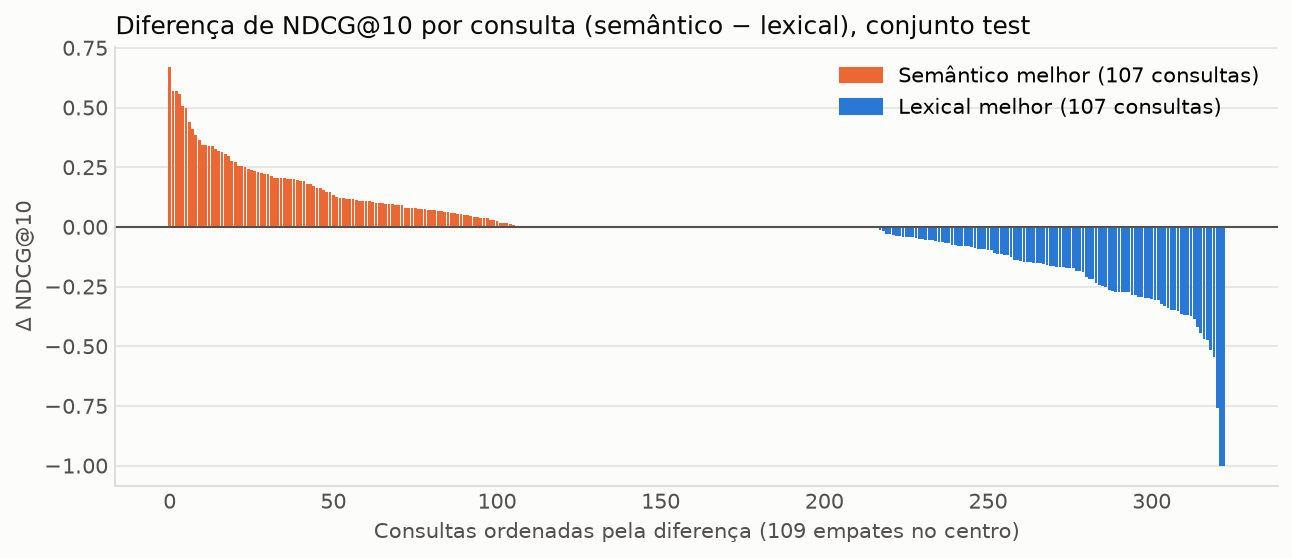
\includegraphics[width=0.86\linewidth]{grafico_delta_lexical_semantico.png}
\caption{Diferença de NDCG@10 por consulta (semântico menos lexical) no conjunto \cod{test}.}
\label{fig:delta}
\end{figure}

As Tabelas~\ref{tab:top5sem} e~\ref{tab:top5lex} mostram o Top-5 de cada método nas três consultas de maior vantagem de cada sistema, com os scores e o grau de relevância. Os valores citados na análise (DF, IDF, parcelas do BM25, posições e subpalavras) foram extraídos dos dados e estão no notebook.

\begin{table}[!htb]
\centering\footnotesize
\setlength{\tabcolsep}{5pt}
\caption{Top-5 nas três consultas de maior vantagem do sistema semântico. Entre parênteses, o NDCG@10 do lexical e do semântico. Rel.: grau de relevância nos qrels (0: não relevante ou não julgado).}
\label{tab:top5sem}
\begin{tabular*}{0.92\linewidth}{@{\extracolsep{\fill}}clrcclcc}
\toprule
 & \multicolumn{3}{c}{Lexical} & & \multicolumn{3}{c}{Semântico} \\
\cmidrule(lr){2-4}\cmidrule(lr){6-8}
Pos. & Documento & BM25 & Rel. & & Documento & Cosseno & Rel. \\
\midrule
\multicolumn{8}{l}{\textbf{PLAIN-307}, \emph{Vitamin D: Shedding some light on the new recommendations} (0,148; 0,819)} \\
1 & MED-3099 & 15,83 & 0 & & MED-714 & 0,742 & 2 \\
2 & MED-4872 & 12,86 & 0 & & MED-3988 & 0,696 & 0 \\
3 & MED-3373 & 12,48 & 0 & & MED-3987 & 0,677 & 0 \\
4 & MED-1579 & 10,63 & 0 & & MED-919 & 0,664 & 2 \\
5 & MED-1777 & 10,37 & 0 & & MED-3990 & 0,648 & 0 \\
\midrule
\multicolumn{8}{l}{\textbf{PLAIN-3085}, \emph{The Difficulty of Arriving at a Vitamin D Recommendation} (0,000; 0,571)} \\
1 & MED-3632 & 10,61 & 0 & & MED-714 & 0,701 & 0 \\
2 & MED-2765 & 9,45 & 0 & & MED-4566 & 0,641 & 0 \\
3 & MED-919 & 9,39 & 0 & & MED-4573 & 0,635 & 2 \\
4 & MED-4872 & 9,17 & 0 & & MED-4570 & 0,617 & 2 \\
5 & MED-4575 & 8,66 & 0 & & MED-919 & 0,611 & 0 \\
\midrule
\multicolumn{8}{l}{\textbf{PLAIN-1537}, \emph{low-carb diets} (0,095; 0,662)} \\
1 & MED-4880 & 20,44 & 0 & & MED-4515 & 0,662 & 1 \\
2 & MED-2943 & 5,70 & 0 & & MED-4880 & 0,609 & 0 \\
3 & MED-1714 & 5,62 & 0 & & MED-4514 & 0,596 & 1 \\
4 & MED-4515 & 5,47 & 1 & & MED-1616 & 0,587 & 1 \\
5 & MED-2458 & 5,46 & 0 & & MED-2586 & 0,558 & 1 \\
\bottomrule
\end{tabular*}
\end{table}

\paragraph{Vantagem do semântico.}
\begin{itemize}
\item \textbf{PLAIN-307.} A expressão \emph{shedding some light} é figurada, mas o BM25 trata \cod{shed} e \cod{light} como termos comuns. O termo \cod{shed} é o mais raro da consulta (DF 13, IDF 5,60) e domina o score: o primeiro colocado, MED-3099, trata de um receptor celular e contém a frase \emph{This concept sheds new light on\ldots}; dos seus 15,83 pontos, 7,52 vêm de \cod{shed}, 5,01 de \cod{light} e 3,29 de \cod{new}, e ele não contém \cod{vitamin}. Além disso, a letra \cod{d} é stopword na lista do NLTK, de modo que \emph{Vitamin D} vira apenas \cod{vitamin}. No semântico, os cinco primeiros são sobre vitamina D, e dois são relevantes de grau 2 (MED-714 e MED-919), que no lexical estavam nas posições 26 e 13.
\item \textbf{PLAIN-3085.} O termo mais raro, \cod{arriv} (DF 7, IDF 6,18), aparece fora de contexto: o primeiro colocado lexical, MED-3632, estuda a mortalidade após a chegada (\emph{arrival}) da pluma radioativa de Fukushima, e todo o seu score (10,61) vem desse termo. Os dois relevantes (MED-4573 e MED-4570) tratam de níveis e doses adequados de vitamina D sem usar \emph{recommendation}, \emph{difficulty} ou \emph{arriving}: contêm apenas \cod{vitamin}. O BM25 os deixa nas posições 40 e 69; o semântico, em 3 e 4. É um caso de variação de vocabulário.
\item \textbf{PLAIN-1537.} A consulta usa a abreviação \emph{carb}, e os artigos escrevem \emph{carbohydrate}. No índice são termos distintos: \cod{carb} tem DF 1 e \cod{carbohydr} tem DF 143, e nenhum dos 45 relevantes contém \cod{carb}. O único documento com o termo (MED-4880) recebe dele 14,80 dos seus 20,44 pontos e fica em primeiro, sem ser relevante; o resto do ranking depende de \cod{low} e \cod{diet}, muito frequentes. O bi-encoder aproxima as duas formas: 4 dos 5 primeiros são relevantes.
\end{itemize}

\begin{table}[!htb]
\centering\footnotesize
\setlength{\tabcolsep}{5pt}
\caption{Top-5 nas três consultas de maior vantagem do sistema lexical. Entre parênteses, o NDCG@10 do lexical e do semântico. Em PLAIN-1473 o BM25 devolve um único documento.}
\label{tab:top5lex}
\begin{tabular*}{0.92\linewidth}{@{\extracolsep{\fill}}clrcclcc}
\toprule
 & \multicolumn{3}{c}{Lexical} & & \multicolumn{3}{c}{Semântico} \\
\cmidrule(lr){2-4}\cmidrule(lr){6-8}
Pos. & Documento & BM25 & Rel. & & Documento & Cosseno & Rel. \\
\midrule
\multicolumn{8}{l}{\textbf{PLAIN-1473}, \emph{kohlrabi} (1,000; 0,000)} \\
1 & MED-4455 & 11,66 & 1 & & MED-3947 & 0,220 & 0 \\
2 & -- & -- & -- & & MED-4660 & 0,217 & 0 \\
3 & -- & -- & -- & & MED-3441 & 0,216 & 0 \\
4 & -- & -- & -- & & MED-3447 & 0,213 & 0 \\
5 & -- & -- & -- & & MED-5024 & 0,212 & 0 \\
\midrule
\multicolumn{8}{l}{\textbf{PLAIN-2081}, \emph{shelf life} (1,000; 0,000)} \\
1 & MED-4303 & 14,68 & 1 & & MED-1378 & 0,415 & 0 \\
2 & MED-1182 & 11,79 & 0 & & MED-2422 & 0,386 & 0 \\
3 & MED-2700 & 10,93 & 0 & & MED-2510 & 0,386 & 0 \\
4 & MED-2671 & 10,52 & 0 & & MED-4715 & 0,382 & 0 \\
5 & MED-2074 & 8,70 & 0 & & MED-1433 & 0,373 & 0 \\
\midrule
\multicolumn{8}{l}{\textbf{PLAIN-1288}, \emph{grapes} (0,890; 0,130)} \\
1 & MED-2668 & 9,40 & 1 & & MED-3200 & 0,426 & 0 \\
2 & MED-2669 & 9,19 & 1 & & MED-398 & 0,425 & 0 \\
3 & MED-2083 & 8,94 & 0 & & MED-3207 & 0,425 & 0 \\
4 & MED-1538 & 8,94 & 1 & & MED-3210 & 0,424 & 0 \\
5 & MED-5065 & 8,73 & 1 & & MED-2083 & 0,414 & 0 \\
\bottomrule
\end{tabular*}
\end{table}

\paragraph{Vantagem do lexical.}
\begin{itemize}
\item \textbf{PLAIN-1473.} O termo \cod{kohlrabi} ocorre em um único documento da coleção, que é o único relevante, e o BM25 devolve exatamente esse documento. O bi-encoder não tem representação útil para a palavra: o tokenizador a quebra em \cod{ko}+\cod{hl}+\cod{ra}+\cod{bi}, o cosseno do primeiro colocado é 0,220 (a mediana do \cod{test} é 0,509) e o relevante fica na posição 117 do ranking semântico completo.
\item \textbf{PLAIN-2081.} \emph{Shelf life} (prazo de validade) é uma expressão cujo sentido não é a soma das partes. O bi-encoder a interpreta pelo sentido geral de \emph{life}: entre os cinco primeiros há documentos sobre longevidade e envelhecimento (MED-1378, MED-2510, MED-1433), e nenhum contém \cod{shelf}. No BM25, \cod{shelf} é raro (DF 7, IDF 6,18) e ancora o ranking: o único relevante, MED-4303, fica em primeiro; no semântico ele está na posição 15.
\item \textbf{PLAIN-1288.} Quatro dos cinco primeiros do semântico são sobre \emph{grapefruit} (toranja), outra fruta, e nenhum contém \cod{grape}. O tokenizador divide \emph{grapefruit} em \cod{grape}+\cod{fr}+\cod{uit}, que começa pelo mesmo fragmento da consulta, o que provavelmente aproxima os embeddings. No índice lexical, \cod{grape} (DF 29) e \cod{grapefruit} (DF 22) são termos distintos, e 4 dos 5 primeiros do BM25 são relevantes. A vantagem é de precisão no topo: dos 196 relevantes da consulta, só 15 contêm \cod{grape}.
\end{itemize}

\paragraph{Síntese.} O semântico vence quando consulta e documentos usam palavras diferentes para o mesmo assunto e quando a consulta traz palavras raras que não carregam o tema; nesses casos o IDF alto atrapalha o BM25. O lexical vence quando a consulta é um termo específico que ocorre literalmente em poucos documentos. O bi-encoder falhou de três formas: palavra rara sem representação própria, expressão composta interpretada pelo sentido mais comum e confusão com uma palavra de grafia parecida. Uma ressalva: os qrels do NFCorpus foram extraídos automaticamente das ligações entre as páginas do site NutritionFacts.org e os artigos citados~\cite{boteva2016}, de modo que relevância 0 inclui documentos nunca julgados, como os artigos sobre vitamina D no Top-5 semântico da PLAIN-307.

\FloatBarrier
\subsection{Busca híbrida}

No \cod{dev}, os três valores de $k$ ficam muito próximos (Tabela~\ref{tab:rrf}); pelo critério definido, usamos $k=10$. No \cod{test} (Tabela~\ref{tab:geral}), o híbrido supera os dois sistemas nas quatro métricas: o NDCG@10 é de 0,3549, 8,2\% acima do lexical e 12,1\% acima do semântico.

\begin{table}[!htb]
\centering\small
\caption{Ajuste de $k$ do RRF no conjunto \cod{dev}. Referência: lexical 0,2959 e semântico 0,3024 de NDCG@10.}
\label{tab:rrf}
\begin{tabular}{ccccc}
\toprule
$k$ & P@10 & R@10 & MAP@10 & NDCG@10 \\
\midrule
10 & 0,2623 & 0,1482 & 0,1064 & \textbf{0,3307} \\
60 & 0,2611 & 0,1508 & 0,1065 & 0,3291 \\
100 & 0,2630 & 0,1510 & 0,1066 & 0,3304 \\
\bottomrule
\end{tabular}
\end{table}

A fusão funciona porque os rankings são complementares: em média, lexical e semântico têm só 2,9 documentos em comum no Top-10 (22,8 no Top-100). Um documento presente nos dois rankings soma duas parcelas e sobe. Por consulta, o híbrido fica acima dos dois sistemas em 51 casos, iguala o melhor em 136, fica entre os dois em 117 e abaixo de ambos em apenas 6. A fusão raramente é pior que os dois sistemas, mas não escolhe o melhor de cada consulta. Nas seis consultas da seção anterior, ela preserva boa parte do resultado do sistema que acertou (0,733 em PLAIN-307 e 1,000 em \emph{shelf life}), mas o sistema que falhou injeta documentos irrelevantes no topo: em \emph{low-carb diets} o híbrido fica em 0,385, contra 0,662 do semântico. Nas 15 consultas sem resultado lexical, o híbrido é idêntico ao semântico. O custo da fusão é desprezível (0,06~ms por consulta).

\FloatBarrier
\subsection{Reranking}

\paragraph{Escolha do modelo.} No \cod{dev} (Tabela~\ref{tab:cedev}), o \cod{ms-marco-MiniLM-L6-v2} tem o maior NDCG@10 e foi adotado, embora o ganho sobre o híbrido sem reranking seja de apenas 0,001. O \cod{TinyBERT-L2} é cerca de 14 vezes mais rápido, mas piora o ranking híbrido: o modelo de 2 camadas não é preciso o bastante para reordenar candidatos que já passaram por dois sistemas.

\begin{table}[!htb]
\centering\small
\caption{Cross-encoders no conjunto \cod{dev}, reordenando os 50 primeiros do híbrido. Tempo médio por consulta em CPU.}
\label{tab:cedev}
\begin{tabular}{lccccc}
\toprule
Modelo & P@10 & R@10 & MAP@10 & NDCG@10 & Tempo \\
\midrule
Híbrido sem reranking & 0,2623 & 0,1482 & 0,1064 & 0,3307 & -- \\
\cod{ms-marco-TinyBERT-L2-v2} & 0,2580 & 0,1494 & 0,1073 & 0,3252 & 0,35 s \\
\cod{ms-marco-MiniLM-L6-v2} & 0,2620 & 0,1548 & 0,1086 & \textbf{0,3317} & 4,86 s \\
\bottomrule
\end{tabular}
\end{table}

O modelo escolhido é o \cod{cross-encoder/ms-marco-MiniLM-L6-v2} (revisão \cod{233902d25c}), com entrada máxima de 512 tokens. No \cod{test}, 1.424 dos 16.150 pares (consulta, documento) passam desse tamanho (8,8\%) e têm o final do documento truncado.

\paragraph{Resultado no \cod{test} e tempos.} O reranking leva o NDCG@10 de 0,3549 para 0,3564 e o MAP@10 de 0,1353 para 0,1389, mas reduz P@10 e R@10 (Tabela~\ref{tab:geral} e Figura~\ref{fig:sistemas}). O custo está na Tabela~\ref{tab:tempos}: o reranking responde por cerca de 97\% do tempo do pipeline. Neste hardware e nesta coleção, é a etapa mais cara e a de menor retorno em qualidade de ranking; quase todo o ganho sobre os sistemas isolados vem da fusão.

\begin{figure}[!htb]
\centering
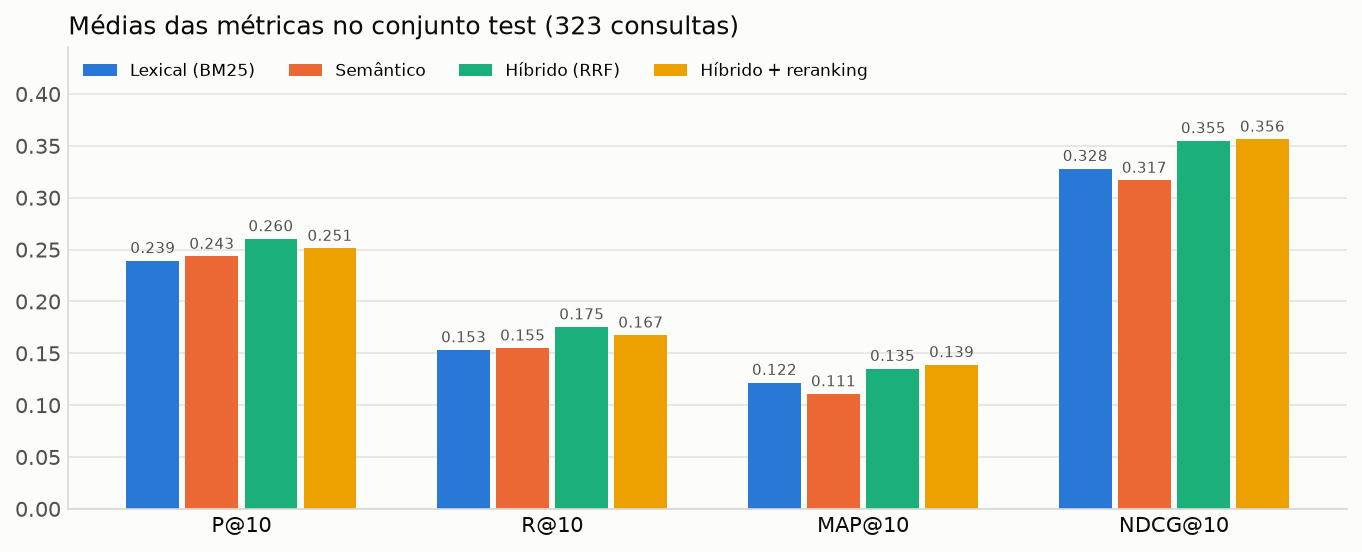
\includegraphics[width=0.82\linewidth]{grafico_comparacao_sistemas.png}
\caption{Médias das métricas no conjunto \cod{test} para os quatro sistemas.}
\label{fig:sistemas}
\end{figure}

\begin{table}[!htb]
\centering\small
\caption{Tempo médio por consulta de cada etapa (CPU, 323 consultas do \cod{test}) e tempo médio de geração por resposta.}
\label{tab:tempos}
\begin{tabular}{lr}
\toprule
Etapa & Tempo médio \\
\midrule
Busca lexical (pré-processamento da consulta + BM25) & 0,26 ms \\
Busca semântica (embedding da consulta + cosseno com 3.633 documentos) & 159,6 ms \\
Fusão (RRF) & 0,06 ms \\
Reranking (50 pares no cross-encoder) & 4.718,6 ms \\
\textbf{Recuperação completa} & \textbf{4.878,6 ms} \\
\midrule
Geração sem RAG (prompt de 46 tokens em média) & 7,6 s \\
Geração com RAG (prompt de 2.285 tokens em média) & 85,4 s \\
\bottomrule
\end{tabular}
\end{table}

\paragraph{Análise do reranking.} O reranking melhora 104 consultas, piora 97 e não altera o NDCG@10 de 122. Três fatos explicam o saldo quase nulo. Primeiro, ele melhora a primeira posição, mas não o Top-10: as consultas com um relevante em primeiro lugar passam de 155 para 165, enquanto a média de relevantes no Top-10 cai de 2,60 para 2,51. Como NDCG e AP dão mais peso ao topo, sobem um pouco, e as métricas que só contam relevantes descem. Segundo, o efeito depende do tipo de consulta (Tabela~\ref{tab:cetipo}): o cross-encoder foi treinado com perguntas em linguagem natural do MS MARCO, ajuda nas consultas longas e nas perguntas e atrapalha nas consultas de uma palavra, que são um terço do \cod{test}. Terceiro, há um teto: em média só 6,1 relevantes estão entre os 50 candidatos, e em 55 consultas não há nenhum.

\begin{table}[!htb]
\centering\small
\caption{Efeito do reranking sobre o NDCG@10 por tipo de consulta (\cod{test}).}
\label{tab:cetipo}
\begin{tabular}{lrccccc}
\toprule
Tipo de consulta & Consultas & Híbrido & Reranking & Diferença & Melhorou & Piorou \\
\midrule
1 palavra & 103 & 0,4006 & 0,3922 & $-$0,0084 & 22 & 27 \\
2 ou 3 palavras & 89 & 0,3397 & 0,3429 & $+$0,0033 & 29 & 27 \\
4 ou mais palavras & 131 & 0,3292 & 0,3373 & $+$0,0080 & 53 & 43 \\
\midrule
Em forma de pergunta & 42 & & & $+$0,0094 & & \\
Demais & 281 & & & $+$0,0003 & & \\
\bottomrule
\end{tabular}
\end{table}

A Tabela~\ref{tab:cecasos} resume os quatro casos pedidos: os dois de maior ganho, um sem alteração (entre as consultas de menor diferença absoluta, a de maior NDCG@10 no híbrido) e o de maior piora.

\begin{table}[!htb]
\centering\footnotesize
\setlength{\tabcolsep}{5pt}
\caption{Principais documentos que mudaram de posição nos quatro casos analisados. CE: score do cross-encoder.}
\label{tab:cecasos}
\begin{tabular}{llccrl}
\toprule
Caso (NDCG@10: híbrido $\rightarrow$ reranking) & Documento & Rel. & Posição & CE & Conteúdo \\
\midrule
PLAIN-1320, \emph{Harvard Physicians' Study II} & MED-2760 & 1 & 11 $\rightarrow$ 1 & 0,76 & artigo do estudo \\
(0,000 $\rightarrow$ 0,562) & MED-2758 & 1 & 12 $\rightarrow$ 3 & $-$2,01 & artigo do estudo \\
 & MED-2761 & 1 & 19 $\rightarrow$ 6 & $-$5,36 & artigo do estudo \\
 & MED-2112 & 0 & 1 $\rightarrow$ 28 & $-$9,77 & médicos em geral \\
\midrule
PLAIN-1473, \emph{kohlrabi} & MED-4455 & 1 & 2 $\rightarrow$ 1 & 1,22 & contém o termo \\
(0,631 $\rightarrow$ 1,000) & MED-3947 & 0 & 1 $\rightarrow$ 20 & $-$9,14 & hibisco \\
\midrule
PLAIN-1039, \emph{domoic acid} & MED-4380 & 1 & 1 $\rightarrow$ 1 & 7,94 & ácido domoico \\
(1,000 $\rightarrow$ 1,000) & MED-4381 & 1 & 2 $\rightarrow$ 2 & 4,93 & ácido domoico \\
 & MED-4995 & 0 & 3 $\rightarrow$ 3 & $-$3,63 & ácido salicílico \\
\midrule
PLAIN-1679, \emph{myelopathy} & MED-5142 & 1 & 5 $\rightarrow$ 40 & $-$10,20 & degeneração da medula \\
(0,387 $\rightarrow$ 0,000) & MED-1105 & 0 & 32 $\rightarrow$ 1 & 0,19 & mieloma múltiplo \\
 & MED-1104 & 0 & 24 $\rightarrow$ 2 & $-$0,93 & mieloma múltiplo \\
\bottomrule
\end{tabular}
\end{table}

\begin{itemize}
\item \textbf{Ganho, PLAIN-1320.} A consulta é o nome de um estudo. No híbrido, o topo era de documentos sobre médicos em geral, trazidos pelo semântico. O lexical tinha os artigos do estudo nas posições 3, 5 e 7, mas eles estavam mal colocados no semântico (74, 38 e 84), e a fusão os deixou em 11, 12 e 19. O cross-encoder lê consulta e documento juntos e reconhece o nome do estudo nos títulos (\emph{\ldots The Physicians' Health Study II Randomized Controlled Trial}). Os pares desses documentos têm de 651 a 754 tokens e foram truncados, sem prejuízo, porque o nome está no título.
\item \textbf{Ganho, PLAIN-1473.} O único relevante estava em segundo no híbrido por um empate de RRF com o primeiro do semântico (ambos valem $1/11$). O cross-encoder lhe dá o único score positivo da lista, porque a palavra da consulta aparece no documento. Ele enxerga a correspondência exata que o bi-encoder não captou.
\item \textbf{Sem alteração, PLAIN-1039.} Os dois únicos relevantes já eram primeiro e segundo no lexical, no semântico e no híbrido, e o cross-encoder confirma a ordem com folga. Abaixo deles a ordem dos não relevantes muda, sem efeito na métrica. Quando os recuperadores concordam e um termo técnico raro identifica os documentos, o reranking não tem o que acrescentar.
\item \textbf{Piora, PLAIN-1679.} \emph{Myelopathy} não ocorre na coleção, e os candidatos vêm só do semântico, que tinha o único relevante em quinto. Esse documento descreve um caso de mielopatia (\emph{degeneration of the spinal cord}) sem usar a palavra da consulta, recebe score $-$10,20 e cai para a posição 40. Sobem documentos sobre mieloma múltiplo: para o tokenizador do cross-encoder, \emph{myelopathy} é \cod{my}+\cod{elo}+\cod{pathy} e \emph{myeloma} é \cod{my}+\cod{elo}+\cod{ma}. O modelo premiou a semelhança de grafia entre dois termos médicos sem relação, o mesmo tipo de confusão de \emph{grapes} e \emph{grapefruit}.
\end{itemize}

\FloatBarrier
\subsection{RAG: recuperação e geração}
\label{sec:res-rag}

A Tabela~\ref{tab:rag} traz, para as 10 consultas, as métricas de recuperação do contexto e as notas das respostas nas duas condições. O maior prompt da condição com RAG teve 2.931 tokens, dentro da janela de 8.192: nenhum contexto foi truncado.

\begin{table}[!htb]
\centering\footnotesize
\setlength{\tabcolsep}{3pt}
\caption{Experimento sem RAG (A) e com RAG (B). Rel.: relevantes no contexto (de 5). Notas de 0 a 2 em fidelidade, completude, utilidade e rastreabilidade (esta última só se aplica a B).}
\label{tab:rag}
\begin{tabular}{llcccccccccc}
\toprule
 & & \multicolumn{3}{c}{Recuperação} & \multicolumn{2}{c}{Fidel.} & \multicolumn{2}{c}{Compl.} & \multicolumn{2}{c}{Util.} & Rastr. \\
\cmidrule(lr){3-5}\cmidrule(lr){6-7}\cmidrule(lr){8-9}\cmidrule(lr){10-11}\cmidrule(lr){12-12}
Consulta & Pergunta & Rel. & P@5 & R@5 & A & B & A & B & A & B & B \\
\midrule
PLAIN-68 & What is Actually in Chicken Nuggets? & 1 & 0,2 & 0,018 & 0 & 2 & 1 & 2 & 1 & 2 & 2 \\
PLAIN-2450 & Are Organic Foods Safer? & 2 & 0,4 & 0,053 & 1 & 1 & 1 & 2 & 2 & 2 & 2 \\
PLAIN-153 & How Should I Take Probiotics? & 5 & 1,0 & 0,106 & 1 & 2 & 1 & 2 & 1 & 2 & 2 \\
PLAIN-2850 & More Antibiotics In White Meat or Dark Meat? & 0 & 0,0 & 0,000 & 0 & 2 & 1 & 0 & 1 & 0 & 1 \\
PLAIN-2750 & Preventing the Common Cold with Probiotics? & 4 & 0,8 & 0,068 & 1 & 2 & 1 & 1 & 1 & 2 & 2 \\
PLAIN-270 & Is Caffeinated Tea Really Dehydrating? & 2 & 0,4 & 0,038 & 1 & 2 & 1 & 2 & 1 & 2 & 2 \\
PLAIN-2470 & Is Milk Good for Our Bones? & 3 & 0,6 & 0,041 & 0 & 2 & 1 & 2 & 1 & 2 & 1 \\
PLAIN-2430 & Preventing Brain Loss with B Vitamins? & 3 & 0,6 & 0,065 & 1 & 2 & 1 & 2 & 1 & 2 & 0 \\
PLAIN-238 & How Chemically Contaminated Are We? & 1 & 0,2 & 0,019 & 1 & 2 & 1 & 1 & 1 & 1 & 2 \\
PLAIN-3342 & Is Coconut Milk Good For You? & 2 & 0,4 & 0,667 & 1 & 2 & 1 & 1 & 2 & 1 & 2 \\
\midrule
Média & & 2,3 & 0,46 & 0,107 & 0,7 & 1,9 & 1,0 & 1,5 & 1,2 & 1,6 & 1,6 \\
\bottomrule
\end{tabular}
\end{table}

\paragraph{Recuperação.} Em 9 das 10 consultas pelo menos um relevante chegou à LLM (Hit@5 de 0,9), e em média 2,3 dos 5 documentos do contexto são relevantes (P@5 de 0,46). O R@5 médio de 0,107 é baixo por construção: as consultas têm de 3 a 73 relevantes, e mesmo com cinco relevantes em todos os contextos o R@5 médio seria 0,234. O P@5 calculado pelos qrels subestima alguns contextos: em PLAIN-2450, o primeiro documento (MED-1140, \emph{Organic food: buying more safety or just peace of mind?}) trata exatamente da pergunta e não tem julgamento.

\paragraph{Geração.} \completar{revisar este parágrafo depois da conferência das notas pelos integrantes.} A fidelidade é o critério que mais muda, de 0,7 para 1,9. Sem RAG, a LLM responde de memória, com afirmações genéricas que os documentos da coleção em parte não sustentam; três respostas recebem nota 0. Com RAG, 9 das 10 respostas têm fidelidade 2; a exceção é PLAIN-2450, com um erro factual apesar do documento correto no contexto. Completude (1,0 para 1,5) e utilidade (1,2 para 1,6) melhoram menos. As respostas com RAG tendem a resumir um único documento: 8 das 10 citam exatamente um \cod{doc\_id}, e em 7 delas é o primeiro do contexto, de modo que a ordem produzida pelo reranking pesa no que a LLM responde. Em duas consultas a utilidade caiu com o RAG: em PLAIN-2850 nenhum relevante foi recuperado, e a LLM se absteve; em PLAIN-3342 os documentos tratam de coco em geral, e a LLM declarou falta de evidência sobre leite de coco. A instrução de avisar quando não há evidência torna o modelo mais cauteloso, o que aumenta a fidelidade e pode custar utilidade.

A rastreabilidade média na condição com RAG é 1,6. Sete respostas permitem ligar as afirmações aos \cod{doc\_ids}. Os problemas são de três tipos: nenhuma citação (PLAIN-2430, apesar da instrução do prompt), dado de um documento atribuído a outro (PLAIN-2470) e conclusão sobre o contexto inteiro apoiada em um único documento (PLAIN-2850). Na condição sem RAG não há contexto nem fontes, e a rastreabilidade não se aplica. A consequência prática é que o leitor não tem como verificar a resposta: em PLAIN-2850, a resposta sem RAG afirma, com uma justificativa plausível, o contrário do que mostra o documento relevante da coleção.

São 10 consultas e uma escala de três níveis: as médias indicam tendência, não diferenças estatisticamente estabelecidas. A LLM é um modelo pequeno, e um modelo maior provavelmente responderia melhor sem RAG e combinaria melhor vários documentos com RAG.

\FloatBarrier
\subsection{Análise de falhas ponta a ponta}

Os três casos foram escolhidos pela diferença entre as somas das notas de fidelidade, completude e utilidade nas duas condições. A Tabela~\ref{tab:estagios} mostra quantos relevantes cada estágio colocou no Top-5.

\begin{table}[!htb]
\centering\small
\caption{Relevantes no Top-5 em cada estágio, nos três casos analisados (soma das notas: A $\rightarrow$ B).}
\label{tab:estagios}
\begin{tabular}{lcccc}
\toprule
Caso & Lexical & Semântico & Híbrido & Reranking (contexto) \\
\midrule
PLAIN-2470, o RAG melhorou claramente (2 $\rightarrow$ 6) & 2 & 4 & 4 & 3 \\
PLAIN-2450, pouca diferença (4 $\rightarrow$ 5) & 1 & 1 & 1 & 2 \\
PLAIN-2850, o RAG não ajudou (2 $\rightarrow$ 2) & 0 & 0 & 0 & 0 \\
\bottomrule
\end{tabular}
\end{table}

\paragraph{O RAG melhorou claramente: PLAIN-2470, \emph{Is Milk Good for Our Bones?}} Todos os estágios funcionaram. A meta-análise sobre leite e fratura de quadril (MED-1337) é o segundo documento no lexical e o primeiro no semântico, no híbrido e após o reranking, e os três primeiros documentos do contexto são relevantes de grau 2. O reranking trouxe um deles da 12\textsuperscript{a} posição, mas também tirou do Top-5 dois relevantes de grau 1 e pôs no lugar dois documentos que falam de leite em outro contexto. Sem RAG, a LLM dá a resposta convencional (\emph{Yes, milk is good for bones}), que os documentos não sustentam. Com RAG, a resposta se inverte e relata a evidência: não há associação entre consumo de leite e fratura de quadril em mulheres. A ressalva é de atribuição: a resposta cita apenas o MED-1337, mas o dado sobre risco 9\% maior em homens vem do MED-1340 e se refere ao consumo de leite na adolescência.

\paragraph{Pouca diferença: PLAIN-2450, \emph{Are Organic Foods Safer?}} Os cinco documentos do contexto tratam do tema, e o título de um deles é praticamente a própria pergunta. A resposta sem RAG já chegava à conclusão que os documentos sustentam (alimento orgânico não é garantia de segurança). Quando o conhecimento geral do modelo coincide com a literatura, o RAG tem pouco a acrescentar: aqui, acrescentou detalhes e fontes. Também introduziu um erro: a resposta afirma que o produto orgânico tem menor risco de contaminação por \emph{E. coli}, e o MED-1178 diz que esse risco não diferiu. A informação correta estava no contexto, e o erro é da geração.

\paragraph{O RAG não ajudou: PLAIN-2850, \emph{More Antibiotics In White Meat or Dark Meat?}} A informação necessária não chegou ao contexto (Hit@5 nulo). O documento que responde à pergunta é o MED-4166 (grau 2), que mediu resíduos de um antibiótico no músculo do peito e da coxa de frangos. A Tabela~\ref{tab:falha} acompanha esse documento estágio por estágio.

\begin{table}[!htb]
\centering\small
\caption{Percurso do documento relevante MED-4166 na consulta PLAIN-2850.}
\label{tab:falha}
\begin{tabular}{lcp{10.2cm}}
\toprule
Estágio & Posição & Evidência \\
\midrule
Lexical & 191 & O documento diz \emph{breast} e \emph{thigh} e não contém \cod{white}, \cod{dark} nem \cod{meat}. Só \cod{antibiot} casa (BM25 de 6,95; o 100\textsuperscript{o} colocado tem 8,35). Quatro dos cinco documentos do contexto vieram das seis primeiras posições do lexical. \\
Semântico & 14 & Cosseno de 0,478 (o primeiro colocado tem 0,555). \\
Fusão & 39 & Presente em um único ranking: $1/(10+14)=0{,}0417$. O quinto colocado tem 0,0929, e um documento de um só ranking soma no máximo 0,0909. \\
Reranking & 19 & Score de $-$8,25 (o quinto colocado tem $-$6,15). O par tem 333 tokens: não houve truncamento. \\
Contexto & fora & O corte é de 5 documentos. \\
Geração & -- & Com RAG, a LLM declara que o contexto não permite responder. \\
\bottomrule
\end{tabular}
\end{table}

A falha principal é da recuperação lexical, por descasamento de vocabulário: a consulta diz \emph{white meat} e \emph{dark meat}, e o documento diz \emph{breast} e \emph{thigh}. Além de perder o relevante, o lexical encheu o topo com documentos que usam \cod{meat} e \cod{white} em outro sentido (consumo de carne branca e risco de câncer). O semântico reconhece parte da relação, mas a fusão agrava a situação: com $k=10$, nenhum documento exclusivo do semântico poderia chegar ao Top-5 nesta consulta. O reranking recupera 20 posições e também não liga os dois vocabulários; todos os scores do Top-5 são negativos, sinal de que o próprio cross-encoder não viu nenhum candidato claramente relevante. A geração se comportou como instruído: com RAG, a LLM não inventou e se absteve. Sem RAG, respondeu com segurança que a carne escura tem mais resíduos, e o MED-4166 relata o oposto (concentrações maiores no peito do que na coxa). O RAG não melhorou a resposta, mas trocou uma afirmação errada e impossível de verificar por uma abstenção honesta.

Um segundo tipo de falha aparece em PLAIN-3342: dois dos três relevantes chegaram ao contexto (R@5 de 0,667, o maior do experimento) e a resposta com RAG não foi melhor. Ali a recuperação fez o que os qrels pedem, e o limite está no conteúdo disponível na coleção e na cautela da geração.

% ------------------------------- Conclusões --------------------------------
\FloatBarrier
\section{Considerações finais}
\label{sec:conclusao}

\begin{itemize}
\item \textbf{Busca lexical.} O índice invertido implementado do zero responde a uma consulta em menos de 1~ms, e o BM25 chega a NDCG@10 de 0,3280, próximo do valor de referência do BEIR. O limite é a dependência do termo exato: 15 consultas não devolvem nada, e abreviações e sinônimos derrubam o ranking.
\item \textbf{Tolerância a erros.} A correção com bigramas, Jaccard e distância de edição recuperou toda a perda nas 8 consultas afetadas pelo erro e acerta 81\% dos erros sintéticos no \cod{dev}. As transposições são o ponto fraco, e o método não distingue um erro de um termo ausente da coleção. Os embeddings são mais robustos ao erro, mas não imunes.
\item \textbf{Busca semântica.} Tem desempenho global parecido com o do BM25 e acerta consultas diferentes: ganha quando há variação de vocabulário e perde em termos raros e específicos.
\item \textbf{Busca híbrida.} A fusão por RRF é o componente de melhor custo-benefício: ganho de 8,2\% a 12,1\% de NDCG@10 sobre os sistemas isolados, com custo de tempo desprezível.
\item \textbf{Reranking.} O ganho é marginal (0,0015 de NDCG@10) e custa cerca de 97\% do tempo do pipeline em CPU. O cross-encoder melhora a primeira posição e as consultas em forma de pergunta, e piora as consultas de uma palavra.
\item \textbf{RAG.} O contexto recuperado tornou as respostas mais fiéis (0,7 para 1,9) e rastreáveis, mas não é garantia: houve erro de leitura de um documento que estava no contexto, atribuição ao documento errado, abstenção quando a recuperação falhou e uma resposta sem citação.
\item \textbf{Interação entre os componentes.} As falhas se propagam. No caso da PLAIN-2850, o descasamento de vocabulário no lexical tirou o documento relevante do Top-100, a fusão o rebaixou por estar em um único ranking, o reranking o recuperou só em parte, e a LLM ficou sem a informação. As médias não mostram esse encadeamento; ele só aparece quando se acompanha uma consulta de ponta a ponta.
\end{itemize}

As conclusões valem para uma única coleção, com qrels derivados de links e consultas muito curtas. A avaliação do RAG usa 10 consultas e uma LLM pequena, e os tempos foram medidos em CPU.

% ------------------------------- Uso de IA ---------------------------------
\section{Uso de ferramentas de IA}

\textbf{IA como componente do experimento}, documentada na metodologia: os bi-encoders \cod{all-MiniLM-L6-v2} e \cod{multi-qa-MiniLM-L6-cos-v1}, os cross-encoders \cod{ms-marco-MiniLM-L6-v2} e \cod{ms-marco-TinyBERT-L2-v2}, e a LLM \cod{Qwen2.5-3B-Instruct}.

\textbf{IA como apoio ao desenvolvimento}: Claude (Anthropic), via Claude Code, foi usado na implementação do notebook a partir do enunciado (reaproveitando o pré-processamento e a fórmula do BM25 do TP1), na execução dos experimentos, na conferência dos resultados, na redação das análises, do README e deste relatório, e na pré-avaliação das respostas do RAG. \completar{confirmar que as notas foram revisadas pelos integrantes e indicar outros usos de IA pelo grupo, se houver.}

Os integrantes são responsáveis por compreender integralmente o código, a metodologia, as decisões e os resultados apresentados.

% ------------------------------- Referências -------------------------------
\begin{thebibliography}{99}\small

\bibitem{boteva2016} BOTEVA, V.; GHOLIPOUR, D.; SOKOLOV, A.; RIEZLER, S. A Full-Text Learning to Rank Dataset for Medical Information Retrieval. In: \emph{European Conference on Information Retrieval (ECIR)}, 2016.

\bibitem{cormack2009} CORMACK, G. V.; CLARKE, C. L. A.; BÜTTCHER, S. Reciprocal Rank Fusion outperforms Condorcet and individual Rank Learning Methods. In: \emph{ACM SIGIR}, 2009.

\bibitem{jarvelin2002} JÄRVELIN, K.; KEKÄLÄINEN, J. Cumulated gain-based evaluation of IR techniques. \emph{ACM Transactions on Information Systems}, v. 20, n. 4, 2002.

\bibitem{jiao2020} JIAO, X. et al. TinyBERT: Distilling BERT for Natural Language Understanding. In: \emph{Findings of EMNLP}, 2020.

\bibitem{lewis2020} LEWIS, P. et al. Retrieval-Augmented Generation for Knowledge-Intensive NLP Tasks. In: \emph{NeurIPS}, 2020.

\bibitem{macavaney2022} MACAVANEY, S.; MACDONALD, C.; OUNIS, I. Streamlining Evaluation with ir-measures. In: \emph{European Conference on Information Retrieval (ECIR)}, 2022.

\bibitem{manning2008} MANNING, C. D.; RAGHAVAN, P.; SCHÜTZE, H. \emph{Introduction to Information Retrieval}. Cambridge University Press, 2008.

\bibitem{nogueira2019} NOGUEIRA, R.; CHO, K. Passage Re-ranking with BERT. \emph{arXiv:1901.04085}, 2019.

\bibitem{porter1980} PORTER, M. F. An algorithm for suffix stripping. \emph{Program}, v. 14, n. 3, 1980.

\bibitem{qwen2024} QWEN TEAM. Qwen2.5 Technical Report. \emph{arXiv:2412.15115}, 2024.

\bibitem{reimers2019} REIMERS, N.; GUREVYCH, I. Sentence-BERT: Sentence Embeddings using Siamese BERT-Networks. In: \emph{EMNLP-IJCNLP}, 2019.

\bibitem{robertson2009} ROBERTSON, S.; ZARAGOZA, H. The Probabilistic Relevance Framework: BM25 and Beyond. \emph{Foundations and Trends in Information Retrieval}, v. 3, n. 4, 2009.

\bibitem{thakur2021} THAKUR, N. et al. BEIR: A Heterogeneous Benchmark for Zero-shot Evaluation of Information Retrieval Models. In: \emph{NeurIPS Datasets and Benchmarks}, 2021.

\bibitem{wang2020} WANG, W. et al. MiniLM: Deep Self-Attention Distillation for Task-Agnostic Compression of Pre-Trained Transformers. In: \emph{NeurIPS}, 2020.

\end{thebibliography}

\end{document}
